\documentclass[submit]{../harvardml}


\course{CS1810-S25}
\assignment{Assignment \#1}
\duedate{11:59pm ET, February 14, 2025} 

\usepackage[OT1]{fontenc}
\usepackage[colorlinks,citecolor=blue,urlcolor=blue]{hyperref}
\usepackage{graphicx}
\usepackage{caption}
\usepackage{enumitem}
\usepackage{soul}
\usepackage{amsmath}
\usepackage{amssymb}
\usepackage{color}
\usepackage{todonotes}
\usepackage{listings}
\usepackage{../common}
\usepackage{framed}
\usepackage{float}
\usepackage{ifthen}
\usepackage{bm}

\usepackage[mmddyyyy,hhmmss]{datetime}

\definecolor{verbgray}{gray}{0.9}

\lstnewenvironment{csv}{
  \lstset{backgroundcolor=\color{verbgray},
  frame=single,
  framerule=0pt,
  basicstyle=\ttfamily,
  columns=fullflexible}}{}

 \DeclareMathOperator*{\limover}{\overline{lim}}

%%%%%%%%%%%%%%%%%%%%%%%%%%%%%%%%%%
%% Solution environment
\usepackage{xcolor}
\usepackage{comment}
\newenvironment{solution}
  {\color{blue}\section*{Solution}}
{}
%%%%%%%%%%%%%%%%%%%%%%%%%%%%%%%%%%



\begin{document}
\begin{center}
  {\Large Homework 1: Regression}\\
\end{center}

\subsection*{Introduction}
This homework is on different three different forms of regression:
kernelized regression, nearest neighbors regression, and linear
regression.  We will discuss implementation and examine their
tradeoffs by implementing them on the same dataset, which consists of
temperature over the past 800,000 years taken from ice core samples.

The folder \verb|data| contains the data you will use for this
problem. There are two files:
\begin{itemize}
  \item \verb|earth_temperature_sampled_train.csv|
  \item \verb|earth_temperature_sampled_test.csv|
\end{itemize}

Each has two columns.  The first column is the age of the ice core
sample.  The second column is the approximate difference in a year's temperature (K)
from the average temperature of the 1,000 years preceding it. The temperatures were retrieved from ice cores in
Antarctica (Jouzel et al. 2007)\footnote{Retrieved from
  \url{https://www.ncei.noaa.gov/pub/data/paleo/icecore/antarctica/epica_domec/edc3deuttemp2007.txt}

  Jouzel, J., Masson-Delmotte, V., Cattani, O., Dreyfus, G., Falourd,
  S., Hoffmann, G., … Wolff, E. W. (2007). Orbital and Millennial
  Antarctic Climate Variability over the Past 800,000 Years.
  \emph{Science, 317}(5839), 793–796. doi:10.1126/science.1141038}.

The following is a snippet of the data file:

\begin{csv}
  # Age, Temperature
  399946,0.51
  409980,1.57
\end{csv}

\noindent And this is a visualization of the full dataset:
\begin{center}
  \includegraphics[width=.8\textwidth]{img_input/sample_graph}
\end{center}
\noindent


\textbf{Due to the large magnitude of the years, we will work in terms
  of thousands of years BCE in these problems.} This is taken care of
for you in the provided notebook.






\subsection*{Resources and Submission Instructions}
If you find that you are having trouble with the first couple
problems, we recommend going over the fundamentals of linear algebra
and matrix calculus (see links on website).  The relevant parts of the
\href{https://github.com/harvard-ml-courses/cs181-textbook/blob/master/Textbook.pdf}{cs181-textbook
  notes are Sections 2.1 - 2.7}.  We strongly recommend reading the
textbook before beginning the homework.

We also encourage you to first read the
\href{http://users.isr.ist.utl.pt/~wurmd/Livros/school/Bishop\%20-\%20Pattern\%20Recognition\%20And\%20Machine\%20Learning\%20-\%20Springer\%20\%202006.pdf}{Bishop
  textbook}, particularly: Section 2.3 (Properties of Gaussian
Distributions), Section 3.1 (Linear Basis Regression), and Section 3.3
(Bayesian Linear Regression). (Note that our notation is slightly
different but the underlying mathematics remains the same!).

\textbf{Please type your solutions after the corresponding problems
  using this \LaTeX\ template, and start each problem on a new page.}
You may find the following introductory resources on \LaTeX\ useful:
\href{http://www.mjdenny.com/workshops/LaTeX_Intro.pdf}{\LaTeX\ Basics}
and
\href{https://www.overleaf.com/learn/latex/Free_online_introduction_to_LaTeX_(part_1)}{\LaTeX\ tutorial
  with exercises in Overleaf}

Homeworks will be submitted through Gradescope. You will be added to
the course Gradescope once you join the course Canvas page. If you
haven't received an invitation, contact the course staff through Ed.

\textbf{Please submit the writeup PDF to the Gradescope assignment
  `HW1'.} Remember to assign pages for each question.

\textbf{Please submit your \LaTeX file and code files to the
  Gradescope assignment `HW1 - Supplemental'.} Your files should be
named in the same way as we provide them in the repository,
e.g. \texttt{hw1.pdf}, etc.

%%%%%%%%%%%%%%%%%%%%%%%%%%%%%%%%%%%%%%%%%%%%%
% Problem 1
%%%%%%%%%%%%%%%%%%%%%%%%%%%%%%%%%%%%%%%%%%%%%
\begin{problem}[kNN and Kernels, 35pts]

You will now implement two non-parametric regressions to model temperatures over time.  
% For this problem, you will use the \textbf{same dataset as in Problem 1}.

\vspace{0.5cm}
\noindent\emph{Make sure to include all required plots in your PDF. Passing all test cases does not guarantee that your solution is correct, and we encourage you to write your own. }

\begin{enumerate}
\item 
 Recall that kNN uses a predictor of the form
\[
  f(x^*) = \frac{1}{k} \sum_n y_n \mathbb{I}(x_n \texttt{ is one of k-closest to } x^*),
\]
where $\mathbb{I}$ is an indicator variable. 
\begin{enumerate}

  \item The kNN implementation \textbf{has been provided for you} in the notebook. Run the cells to plot the results for $k=\{1, 3, N-1\}$, where $N$ is the size of the dataset. Describe how the fits change with $k$. Please include your plot in your solution PDF.

  \item Now, we will evaluate the quality of each model \emph{quantitatively} by computing the error on the provided test set. Write Python code to compute test MSE for each value of $k$.  Which solution has the lowest MSE? 
  
\end{enumerate}

\item \textit{Kernel-based regression} techniques are another form of non-parametric regression. Consider a kernel-based
regressor of the form 
\begin{equation*}
  f_\tau(x^*) = \cfrac{\sum_{n} K_\tau(x_n,x^*) y_n}{\sum_n K_\tau(x_n, x^*)}
\end{equation*}
where $\mathcal{D}_\texttt{train} = \{(x_n,y_n)\}_{n = 1} ^N$ are the
training data points, and $x^*$ is the point for which you want to
make the prediction.  The kernel $K_\tau(x,x')$ is a function that
defines the similarity between two inputs $x$ and $x'$. A popular
choice of kernel is a function that decays as the distance between the
two points increases, such as
\begin{equation*}
  K_\tau(x,x') = \exp\left(-\frac{(x-x')^2}{\tau}\right)
\end{equation*}

where $\tau$ represents the square of the lengthscale (a scalar value that
dictates how quickly the kernel decays).  


\begin{enumerate}
    
  \item First, implement the \texttt{kernel\_regressor} function in the notebook, and plot your model for years in the range $800,000$ BC to $400,000$ BC at $1000$ year intervals for the following three values of $\tau$: $1, 50, 2500$. Since we're working in terms of thousands of years, this means you should plot $(x, f_\tau(x))$ for $x = 400, 401, \dots, 800$. \textbf{In no more than 10 lines}, describe how the fits change with $\tau$. Please include your plot in your solution PDF.

  \item Denote the test set as $\mathcal{D}_\texttt{test} = \{(x'_m, y'_m)\}_{m = 1} ^M$.  Write down the expression for MSE of $f_\tau$ over the test set as a function of the training set and test set. Your answer may include $\{(x'_m, y'_m)\}_{m = 1} ^M$, $\{(x_n, y_n)\}_{n = 1} ^N$, and $K_\tau$, but not $f_\tau$.

    \item Compute the MSE on the provided test set for the three values of $\tau$.  Which model yields the lowest MSE? Conceptually, why is this the case? Why would choosing $\tau$ based on $\mathcal{D}_\texttt{train}$ rather than $\mathcal{D}_\texttt{test}$ be a bad idea? 

  \item Describe the time and space complexity of both kernelized regression and kNN with respect to the size of the training set $N$.  How, if at all, does the size of the model---everything that needs to be stored to make predictions---change with the size of the training set $N$?  How, if at all, do the number of computations required to make a prediction for some input $x^*$ change with the size of the training set $N$?.
  

  \item  What is the exact form of $\lim_{\tau \to 0 }f_\tau(x^*)$?
  \end{enumerate}
\end{enumerate}
\end{problem}

\newpage
\begin{solution}
	\begin{enumerate}
	    \item \begin{enumerate}
	        \item The fit of our predictions corresponds very closely as $k$ decreases. At $k=1$, we see that our predictions follow the nearest neighbour (and is overfit), and as $k$ increases, our predictions become less strict/correspond less with the data (the variance decreases and the data is underfit).
            \begin{figure}[H]
	        \centering
	        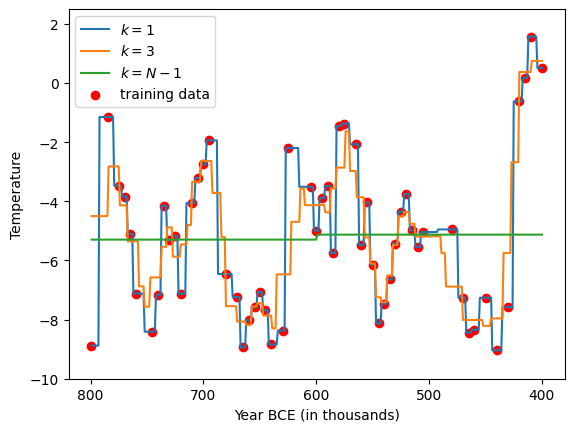
\includegraphics[width=0.5\linewidth]{p1.1a.png}
	    \end{figure}
    
                \item The following is a graph of the MSE for each value of $k$.
                \begin{figure}[H]
                    \centering
                    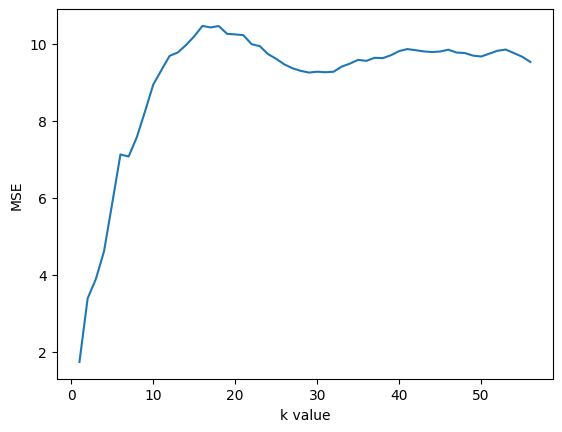
\includegraphics[width=0.5\linewidth]{p1.2.png}
                \end{figure}

                The solution where $k=1$ has the lowest MSE of around $1.7406$.
                
	       \end{enumerate}
        \item 
        \begin{enumerate}
            \item Plot:
            \begin{figure}[H]
                \centering
                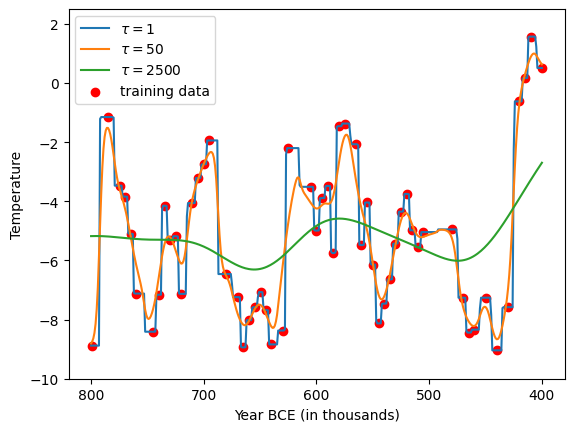
\includegraphics[width=0.5\linewidth]{1.2.1.png}
            \end{figure}

            The fit seems to become "looser" or correspond less closely with the data as $\tau$ increases. At a small $\tau$ (e.g. 1), the kernelized regression has a similar shape as kNN  since distance is weighted heavily. However, as $\tau$ increases, the distance between points is not as strict, so the fit becomes looser with less variance. Therefore, large $\tau$ will weight distant points more than small $\tau$ expressions, so our fit will seemingly transition from overfit-like to underfit as $\tau$ increases. This is evident in the graph above where the $\tau=2500$ line corresponds to the actual datapoints less exact than the line for $\tau=50$. The same relationship exists for $\tau=1$.
            
            \item We know that our expression for MSE for the test dataset will be:

            \[
            \frac{1}{M}\sum_{m=1}^M (y_m' - \hat{y}'_m)^2
            \]

            where our predicted value for $\hat{y}'_m$ is

            \[
            \hat{y}'_m = f_\tau(x'_m) = \cfrac{\sum_{n} K_\tau(x_n,x'_m) y_n}{\sum_n K_\tau(x_n, x'_m)}
            \]

            Thus, we can substitute this into our MSE to find:

            \[
            \boxed{MSE = \frac{1}{M} \sum_{m=1}^{M} \left(y'_m - \cfrac{\sum_{n} K_\tau(x_n,x'_m) y_n}{\sum_n K_\tau(x_n, x'_m)}\right)^2}
            \]

            \item The MSE for the values of $\tau$ are as below:

            \begin{table}[h]
                \centering
                {\color{blue}
                \begin{tabular}{|c|c|}
                    \hline
                    \textbf{Basis Function Part} & \textbf{MSE} \\
                    \hline
                    1 & 1.9473 \\
                    50 & 1.8583 \\
                    2500 & 8.3339 \\
                    \hline
                \end{tabular}}
                \label{tab:mse_values}
            \end{table}

            Out of the three, the model with $\tau = 50$ yields the lowest MSE. Conceptually, this is the case since a very small $\tau$ value would heavily weigh close points while a very high $\tau$ value would weight distance as less important. This corresponds to overfitting and underfitting respectively, so we want to find a "sweet spot" between the two extremes. Thus, conceptually, a $\tau$ value of 50 would likely fit the data better without too many extremes compared to the other values, resulting in a lower MSE.. Choosing a $\tau$ based on the training data would be bad since we would essentially choose a $\tau$ that fits best to that set of data, which would result in overfitting. In other words, if we chose a $\tau$ value based on the training data set, we would just pick the $\tau$ that most closely corresponds to the data.

            \item The time complexity for kernelized regression is $O(N)$ where $N$ is the number of points in the data set. This is because for each prediction, we need to loop through the entire dataset to calculate the weight of a point and value of the point, summing together each point until we get our resulting prediction. In contrast, the time complexity for kNN as it is implemented in the notebook is $O(N\log N)$ since we need to sort the $N$ datapoints based on distance from a point (which optimal sorting takes $O(N\log N)$ time) and then taking the average of the sum of the $k$ points with the smallest distance. (Alternatively, a method such as using quickselect and looping through the list could result in smaller times) \\

            The space complexity for kernelized and kNN are both $O(N)$ since both need to keep track of every data point for each new prediction. This would take $O(N)$ space. This would change in direct proportion to a change in the size of the training set $N$. Similarly, the number of computations to make a prediction would change directly proportional to $N$ as well since the time complexity is in relation to $N$.
            
            \item We can find the exact form of $\lim_{\tau \to 0}f_\tau(x^*)$ in the following. Let $x_c$ be the closest $x$ point to $x^*$. We want to show that $K_\tau(x_c,x^*)$ dominates among all other kernels of other data points. Thus, we see for any $x \neq c$

            \[
            \lim_{\tau \to 0} \frac{K_\tau(x_n, x^*)}{K_\tau (x_c,x^*)} = \exp\left( - \frac{(x_n - x^*)^2 - (x_c-x^*)^2}{\tau} \right)
            \]

            We know that the expression $(x_n - x^*)^2 - (x_c-x^*)^2$ is always positive since by definition $x_c$ is the closest point so $(x_n - x^*)^2 > (x_c-x^*)^2$. Therefore, since $\tau \to 0$, we see that the expression within the $\exp$ will approach $-\infty$. Therefore

            \[
            \lim_{\tau \to 0} \frac{K_\tau(x_n, x^*)}{K_\tau (x_c,x^*)} = 0
            \]

            Thus we see that the term $K_\tau(x_c,x^*)$ dominates the other kernel points. Additionally, we can rewrite the limit as:

            \[
            \lim_{\tau \to 0}\sum_{n} \frac{K_\tau (x_n,x^*)}{\sum_{n}K_\tau (x_n,x^*)}y_n
            \]

            Since $\sum_{n}K_\tau (x_n,x^*) > K_\tau (x_c,x^*)$ as the sum includes the $x_c$ point, we know that the fraction:

            \[
            \frac{K_\tau (x_n,x^*)}{\sum_{n}K_\tau (x_n,x^*)} < \frac{K_\tau(x_n, x^*)}{K_\tau (x_c,x^*)}
            \]

            Therefore, for any $n \neq c$, the values

            \[
            \lim_{\tau\to 0}\frac{K_\tau(x_n,x^*)}{\sum_{n}K_\tau (x_n,x^*)} = 0
            \]

            However, since we know that the fraction

            \[
            \sum_{n} \frac{K_\tau (x_n,x^*)}{\sum_{n}K_\tau (x_n,x^*)} = 1
            \]

            this implies that

            \[
            K_\tau (x_c,x^*) = 1
            \]

            Therefore, we see that the only non-zero point of the sum in the limit will be the result. In other words,

            \[
            \lim_{\tau \to 0}\sum_{n} \frac{K_\tau (x_n,x^*)}{\sum_{n}K_\tau (x_n,x^*)}y_n = y_c
            \]
            
        \end{enumerate}
	\end{enumerate}
\end{solution}


%%%%%%%%%%%%%%%%%%%%%%%%%%%%%%%%%%%%%%%%%%%%%
% Problem 2
%%%%%%%%%%%%%%%%%%%%%%%%%%%%%%%%%%%%%%%%%%%%%
\newpage
\begin{problem}[Deriving Linear Regression, 20pts]

We now seek to model the temperatures with a parametric method: linear regression. Before we implement anything, let's revisit the mathematical formulation of linear regression.  Specifically, the solution for the least squares linear regression  ``looks'' kind of like a ratio of covariance and
variance terms.  In this problem, we will make that connection more
explicit. \\

\noindent Suppose we have some 2-D data where each observation has the form $(x, y)$ and is independent and identically distributed according  $x \sim p(x)$, $y \sim p(y|x)$. We will consider the process of fitting these data from this distribution with the best linear model
possible, that is a linear model of the form $\hat{y} = wx$ that
minimizes the expected squared loss $E_{x,y}[ ( y - \hat{y} )^2
    ]$.\\

\noindent Note: The notation $E_{x, y}$ indicates an
expectation taken over the joint distribution $p(x,y)$. This essentially just means to treat $x$ and $y$ as random.  

\begin{enumerate}

  \item Derive an expression for the optimal $w$, that is, the $w$
        that minimizes the expected squared loss above.  You should leave
        your answer in terms of moments of the distribution, e.g. terms
        like $E_x[x]$, $E_x[x^2]$, $E_y[y]$, $E_y[y^2]$, $E_{x,y}[xy]$
        etc.

  \item Note that while $x, y$ are data that we have access to, $E_{x, y}[yx]$ is a theoretical constant. Keeping in mind the interpretation of expectations as average values, how could you use observed data $\{(x_n,y_n)\}_{n=1}^N$ to estimate $E_{x, y}[yx]$ and $E_x[x^2]$?

  \item In general, moment terms like $E_{x, y}[yx]$, $E_{x, y}[x^2]$,
        $E_{x, y}[yx^3]$, $E_{x, y}[\frac{x}{y}]$, etc. can easily be
        estimated from the data (like you did above).  If you substitute in
        these empirical moments, how does your expression for the optimal
        $w^*$ in this problem compare with the optimal $\bm{\hat w}$ from Problem 4.3 of HW0?

  \item Many common probabilistic linear regression models assume that
        variables $x$ and $y$ are jointly Gaussian.  Did any of your above
        derivations rely on the assumption that $x$ and $y$ are jointly
        Gaussian?  Why or why not?
\end{enumerate}
\end{problem}

\newpage
\begin{solution}
	\begin{enumerate}
	    \item We want to find an expression for the optimal $w$. This can be done by minimizing the expected squared loss $\mathcal{L}(\bm w) = E_{x,y}[ ( y - \hat{y} )^2]$. We can begin by substituting the value of $\hat{y}=wx$ into the expression and simplifying.

        \begin{align*}
            \mathcal{L}(\bm w) &= E_{x,y}[ ( y - \hat{y} )^2] \\
            &=E_{x,y}[ ( y - wx )^2]\\
            &= E_{x,y}[(y^2 - 2wxy + w^2x^2)]\\
            &= E_y[y^2] - E_{x,y}[2wxy] + E_x[w^2x^2] \\
            &= E_y[y^2] - 2wE_{x,y}[xy] + w^2E_x[x^2]
        \end{align*}

        We can take the derivative of this expression with respect to $w$ to find the optimal $w$.

        \[
        \frac{d\mathcal{L}(w)}{dw} = - 2E_{x,y}[xy] + 2wE_x[x^2]
        \]

        By setting the derivative to zero, we can solve for the minimum point of the loss function. This simplifies to

        \[
        2E_{x,y}[xy] = 2wE_x[x^2]
        \]

        Rearranging, we find the optimal $w^*$:

        \[
        \boxed{w^* = \frac{E_{x,y}[xy]}{E_x[x^2]}}
        \]

        \item We can empirically estimate the expected values as averages as the following by the definition of what an average is:

        \[
        \boxed{E_{x,y}[xy] \approx \frac{\sum_{n=1}^N y_n x_n}{N}}
        \]

        \[
        \boxed{E_x[x^2] \approx \frac{\sum_{n=1}^N x_n^2}{N}}
        \]

        Similarly, this empirical method can be applied to any moment terms using the dataset.

        
        \item We can substitute the empirical moments from part 2 into our expression for $w^*$ to get the following:

        \[
        w^* = \frac{\sum_{n=1}^N y_n x_n}{\sum_{n=1}^N x_n^2}
        \]

        From HW0, we have the expression

        \[\bm{\hat w} = (\bm X^\top \bm X)^{-1}\bm X^\top \bm y\]

        We can write the quantity
        
        \[
        \bm X^\top \bm X = \sum_{n=1}^N x_n^2
        \]
        
        since we have 2-D data of the form $(x,y)$ which results in our data having $\bm X$ being formatted as a $N\times1$ vector. Similarly, we can write

        \[
        \bm X^\top \bm y = \sum_{n=1}^N x_ny_n
        \]

        Thus we can see the expression for the optimal $\bm{\hat{w}}$ from HW0 is the same as our empirical optimal $w*$:

        \[
        \bm{\hat w} = \frac{\sum_{n=1}^N y_n x_n}{\sum_{n=1}^N x_n^2} = w^*
        \]

        \item None of the above derivations would rely on the assumption that $x$ and $y$ are jointly Guassian since we do not use properties of a joint Guassian. In our above derivations, we use linearity and moments which do not rely on any prior assumptions regarding a joint nature of $x$ and $y$.        
	\end{enumerate}
\end{solution}

%%%%%%%%%%%%%%%%%%%%%%%%%%%%%%%%%%%%%%%%%%%%%
% Problem 3
%%%%%%%%%%%%%%%%%%%%%%%%%%%%%%%%%%%%%%%%%%%%%

\begin{problem}[Basis Regression, 30pts]

 Having reviewed the theory, we now implement some linear regression models for the temperature. If we just directly use the data as given to us, we would only have
    a one dimensional input to our model, the year.  To create a more expressive linear
    model, we will introduce basis functions.

\vspace{1em}

\noindent\emph{Make sure to include all required plots in your PDF.}

\begin{enumerate}
  \item
        We will first implement the four basis regressions below. (The first basis has been implemented for you in the notebook as an example.) Note that we introduce an addition transform $f$ (already into the provided notebook) to address concerns about numerical instabilities.
        \begin{enumerate}
          \item $\phi_j(x)= f(x)^j$ for $j=1,\ldots, 9$. $f(x) = \frac{x}{1.81 \cdot 10^{2}}.$
          \item $\phi_j(x) = \exp\left\{-\cfrac{(f(x)-\mu_j)^2}{5}\right\}$ for $\mu_j=\frac{j + 7}{8}$ with $j=1,\ldots, 9$. $f(x) = \frac{x}{4.00 \cdot 10^{2}}.$
          \item $\phi_j(x) =  \cos(f(x) / j)$ for $j=1, \ldots, 9$. $f(x) = \frac{x}{1.81}$.
          \item $\phi_j(x) = \cos(f(x) / j)$ for $j=1, \ldots, 49$. $f(x) = \frac{x}{1.81 \cdot 10^{-1}}$. \footnote{For the trigonometric bases (c) and (d), the periodic nature of
                  cosine requires us to transform the data such that the
                  lengthscale is within the periods of each element of our basis.}
        \end{enumerate}

        {\footnotesize * Note: Please make sure to add a bias term for
        all your basis functions above in your implementation of the
        \verb|make_basis|.}

        Let
        $$ \mathbf{\phi}(\mathbf{X}) =
          \begin{bmatrix}
            \mathbf{\phi}(x_1) \\
            \mathbf{\phi}(x_2) \\
            \vdots             \\
            \mathbf{\phi}(x_N) \\
          \end{bmatrix} \in \mathbb{R}^{N\times D}.$$
        You will complete the \verb|make_basis| function which must return
        $\phi(\mathbf{X})$ for each part
        (a) - (d). You do NOT need to submit this
        code in your \LaTeX writeup.

        Then, create a plot of the fitted
        regression line for each basis against a scatter plot
        of the training data. Boilerplate plotting code is provided in the
        notebook---you will only need to finish up a part of it.
        \textbf{All you need to include
          in your writeup for this part are these four plots.}

        \item
          Now we have trained each of our basis regressions. For each basis
          regression, compute the MSE on the test set.  Discuss: do any of the
          bases seem to overfit?  Underfit?  Why?


    \item Briefly describe what purpose the transforms $f$ serve: why are they helpful?

    \item As in Problem 1, describe the space and time complexity of linear regression.  How does what is stored to compute predictions change with the size of the training set $N$ and the number of features $D$?  How does the computation needed to compute the prediction for a new input depend on the size of the training set $N$?  How do these complexities compare to those of the kNN and kernelized regressor?

    \item Briefly compare and constrast the different regressors: kNN,
          kernelized regression, and linear regression (with bases).  Are some
          regressions clearly worse than others?  Is there one best
          regression?  How would you use the fact that you have these multiple
          regression functions?

  \end{enumerate}
  Note:
  Recall that we are using a
  different set of inputs $\mathbf{X}$ for each basis (a)-(d).
  Although it may seem as though this prevents us from being able
  to directly compare the MSE since we are using different data,
  each transformation can be considered as being a part of our model.
  Contrast this with transformations (such as standardization) that cause the variance of the target $\mathbf{y}$ to be different; in these cases the
  MSE can no longer be directly compared.
\end{problem}

\newpage 
\begin{solution}
	\begin{enumerate}
	    \item Below:
        \begin{figure}[H]
	    \centering
	    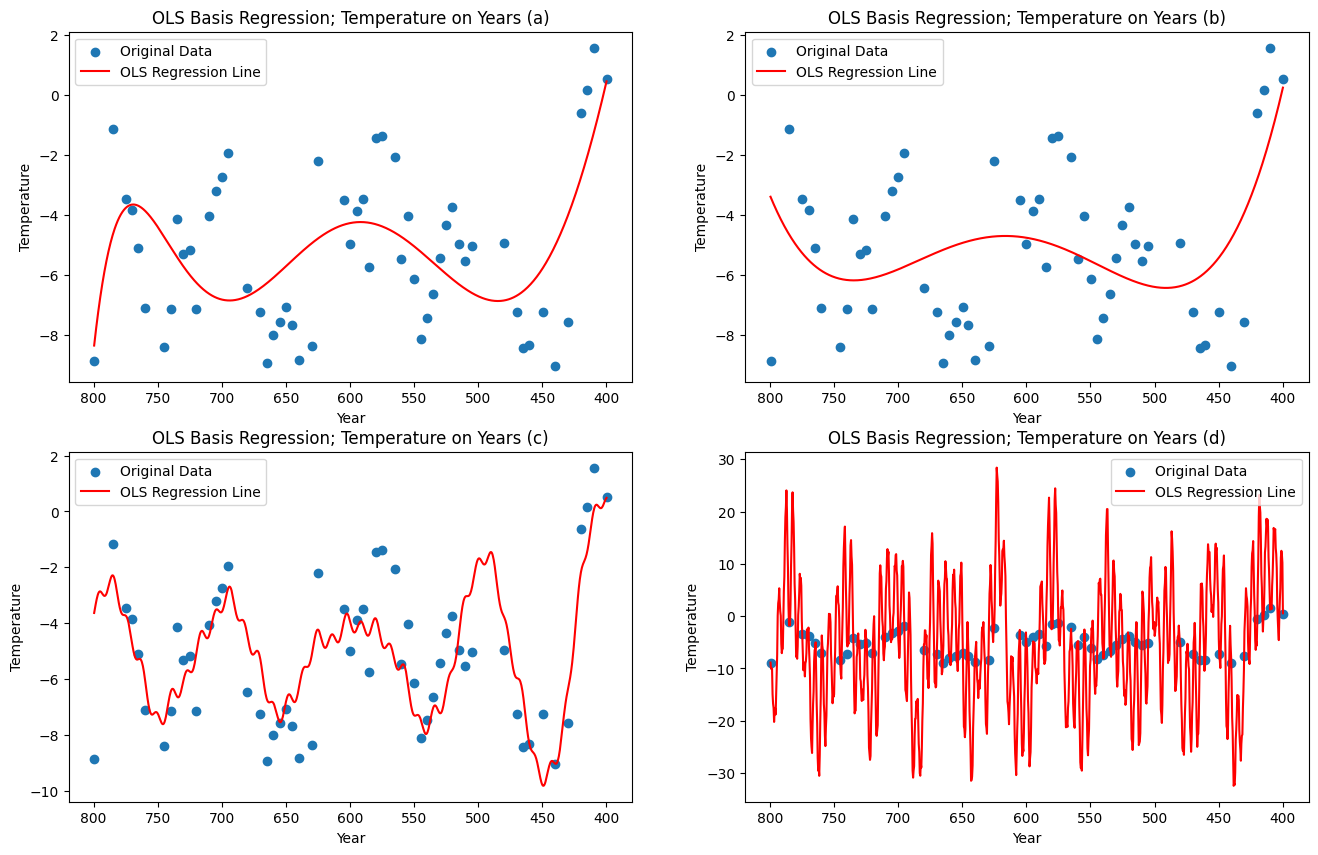
\includegraphics[width=0.8\linewidth]{p3.1.png}
	\end{figure}

        \item The MSE for each of the basis regressions on the test set are bellow:
            \begin{table}[h]
                \centering
                {\color{blue}
                \begin{tabular}{|c|c|}
                    \hline
                    \textbf{Basis Function Part} & \textbf{MSE} \\
                    \hline
                    a & 7.9557 \\
                    b & 8.7082 \\
                    c & 5.9670 \\
                    d & 58.8855 \\
                    \hline
                \end{tabular}}
                \label{tab:mse_values}
            \end{table}

            It seems like $(d)$ overfits on the data as the prediction is very spiky and corresponds very closely to the actual datapoints while having a high MSE value for the test data. In contrast, $(b)$ seems to underfit the data as it has low variance and is not influenced significantly by the datapoints in its predictions with a moderate MSE value on the test data. The basis of $(a)$ could be underfit as we see that $(c)$ has a smaller MSE value, but the extent to which it is underfit is much less than $(b)$. In general, it seems like the bases with higher MSE values tend to overfit/underfit more, depending on the variance within the graphs.
            
        \item The transform $f$ helps address numerical instabilities by scaling the values of $x$ before being input into the basis function. They are helpful in preventing too large or small numbers which could result in imprecise calculations (e.g. large exponential results).

        \item The time complexity of linear regression is $O(D)$ since after training, we only need to multiply an input by the weights and add up each number (from each dimension index) to find our prediction. The space complexity is also $O(D)$ since all we need to store is the weight vector, which has $D$ elements. Thus, in contrast to kernelized and kNN where we needed to use the datapoints to predict a new point, linear regression is faster at predicting datapoints, although training a model is slow. The computation for prediction new inputs and what is stored do not depend on the size of the training set $N$. Since in most cases $D$ will be less than $N$ and would stay constant, we see that linear regression has better complexities compared to kNN and kernelized regressors.

        \item In general, each of the three different regressors have different use cases, though it seems like typically kernelized regression is better than kNN depending on $\tau$ as it has a smaller time complexity while also being less prone to overfitting/having smoother predictions. Linear regression with bases is typically more efficient in terms of time and space complexity for new predictions since after training, we can just find the dot product of the weights and an input to get a prediction. However, we need to use bases for non-linear data in linear regression while in kNN and kernelized regression we do not need to. While kNN is different from kernelized regression, it does nto seem to be clearly worse as depending on $\tau$ we can get vastly different results. There is also no one best regression as each has a different use case. Overall, with the fact that we have multiple regression functions, we can try each one on a dataset and see which perform the best (splitting data into training, validation, and test while using the methods discussed in lecture such as cross validation). This will allow us to determine the best model to use in a given situation.
    
    \end{enumerate}
\end{solution}

%%%%%%%%%%%%%%%%%%%%%%%%%%%%%%%%%%%%%%%%%%%%%
% Problem 4
%%%%%%%%%%%%%%%%%%%%%%%%%%%%%%%%%%%%%%%%%%%%%
\begin{problem}[Probablistic Regression and Regularization, 30pts]

Finally, we will preview Bayesian regression and explore its connection to regularization for linear models. Then, we will fit a regularized model to the temperature data. Although the content is related, you do not need to know the material from the lectures on frequentist model selection and Bayesian model selection to solve this problem.  \\

\noindent Recall that the probabilistic version of linear regression states that 
\[y_n = \boldw^\top\boldx_n + \epsilon_n, \quad \epsilon_n \sim \mathcal{N}(0, \sigma^2)\]
In Bayesian regression, we impose a prior $p(\boldw)$ on the weights and  fit the weights $\boldw$ through maximizing the posterior likelihood
\[p(\boldw | \boldX, \boldy) = \frac{p(\bold y | \boldw, \boldX)p(\boldw)}{p(\boldy | \boldX)}\]
Note: since we maximize with respect to $\boldw$, it suffices to just maximize the numerator.

\begin{enumerate}
    \item Suppose $\boldw \sim \mathcal{N}(\mathbf{0},\frac{\sigma^2}{\lambda}\boldI)$. Show that maximizing the posterior likelihood is equivalent to minimizing 
    \[\mathcal{L}_{ridge}(\boldw) = \frac{1}{2}||\boldy -\bold X\boldw||_2^2 + \frac{\lambda}{2}||\boldw||_2^2.\] 
    Note that minimizing $\mathcal{L}_{ridge}(\boldw)$ is exactly what ridge regression does.
    
    Hint: You don't need to solve for the maximizer/minimizer to show that the optimization problems are equivalent.
    
    \item Solve for the value of $\boldw$ that minimizes $\mathcal L_{ridge}(\boldw)$.

    \item The Laplace distribution has the PDF
   \[L(a,b) =\frac{1}{2b} \exp\left(-\frac{|x - a|}{b}\right)\]
Show that if all $w_d \sim L\left(0,\frac{2\sigma^2}{\lambda}\right)$, maximizing the posterior likelihood is equivalent to minimizing 
\[\mathcal{L}_{lasso}(\boldw) = \frac{1}{2}||\boldy -\bold X\boldw||_2^2  + \frac{\lambda}{2}||\boldw||_1.\] 
Note that minimizing $\mathcal{L}_{lasso}(\boldw)$ is exactly what LASSO regression does.

    \item Why is there no general closed form for the LASSO estimator, i.e. the value of $\boldw$ that minimizes $\mathcal{L}_{ridge}(\boldw)$?

    \item Since there is no general closed form for LASSO, we use numerical methods for estimating $\boldw$. One approach is to use \textit{coordinate descent}, which works as follows: 
    \begin{enumerate}
        \item Initialize $\boldw=\boldw_0$.
        \item For each $d=1, \ldots, D$ do the following 2 steps consecutively:
        \begin{enumerate}
            \item Compute $\rho_d = \tilde{\boldx}_d^\top(\boldy - (\boldX \boldw - w_d \tilde{\boldx}_d))$. We define $\tilde{\boldx}_d$ as the $d$-th column of $\boldX$.

            \item If $d=1$, set $w_1 = \frac{\rho_1}{||\tilde{\boldx}_1||^2_2}$. Otherwise if $d\ne 1$, compute $w_d = \frac{\text{sign}(\rho_d)\max\left\{|\rho_d|-\frac{\lambda}{2}, 0\right\}}{||\tilde{\boldx}_d||^2_2}$.
        \end{enumerate}
        \item Repeat step (b) until convergence or the maximum number of iterations is reached.
    \end{enumerate} 

    Implement the \texttt{find\_lasso\_weights} function according to the above algorithm, letting the max number of iterations be 5000. Then, fit models with $\lambda=1, 10$ to basis (d) from Problem 3, plot the predictions, and compute the MSE's. You will need to do some preprocessing, but a completed helper function for this is already provided. How do the graphs and errors compare to those for the unregularized basis (d) model? 


\end{enumerate}

\end{problem}

\newpage
\begin{solution}
	\begin{enumerate}
	    \item We want to show that maximizing the posterior likelihood is equivalent to the expression in 1. Additionally, since we are maximizing with respect to $\bm w$, it suffices to maximize just the numerator. Thus, we aim to maximize

        \[
        p(\bm y|\bm w, \bm X)p(\bm w)
        \]

        Since $\log$ is a monotonically increasing function, maximizing the $\log$ of the expression is the same as maximizing it when finding optimal $w$.

        \[
        \log  p(\bm y|\bm w, \bm X) + \log p(\bm w)
        \]

        Let us begin with the expression $p(\bm y|\bm w, \bm X)$. We know that 

        \[y_n = \boldw^\top\boldx_n + \epsilon_n, \quad \epsilon_n \sim \mathcal{N}(0, \sigma^2)\]

        so we can write $y_n | \bm w, \bm x_n \sim \mathcal{N}(\bm w^\top \bm x_n, \sigma^2)$. Thus we can write the probability $p(\bm y | \bm w, \bm X)$ as:
        \begin{align*}
            p(\bm y | \bm w, \bm X) &= \prod_{n=1}^{N} p(y_n|\bm w,\bm x_n) \\
            &= \prod_{n=1}^{N} \frac{1}{\sqrt{2\pi \sigma^2}}\exp\{\frac{-(y_n - \bm w^\top \bm x_n)^2}{2\sigma^2}\}
        \end{align*}

        Therefore the $\log$ version would be
        \begin{align*}
            \log  p(\bm y|\bm w, \bm X) &= \sum_{n=1}^N \left[\log \frac{1}{\sqrt{2\pi \sigma^2}}-\frac{(y_n - \bm w^\top \bm x_n)^2}{2\sigma^2}\right]\\
            &= \sum_{n=1}^N -\frac{1}{2}\log(2\pi\sigma^2)-\frac{1}{2\sigma^2}\sum_{n=1}^N(y_n-\bm w^\top \bm x_n)^2 \\
            &= -\frac{N}{2}\log(2\pi\sigma^2)-\frac{1}{2\sigma^2}||\bm y-\bm X \bm w||^2_2
        \end{align*}

        We can take a similar process to expand $p(\bm w)$ where $D$ is the number of dimensions of the vector $\bm w$.

        \[
        p(\bm w) = \frac{1}{(2\pi)^{D/2}\left|\frac{\sigma^2}{\lambda}\bm I\right|^{\frac{1}{2}}}\exp\{-\frac{1}{2}\bm w^\top \left(\frac{\sigma^2}{\lambda}\bm I\right)^{-1}\bm w\}
        \]

        Since the covariance matrix is just a diagonal with each diagonal element being $\frac{\sigma^2}{\lambda}$, the determinant can be found as
        \[
        \left|\frac{\sigma^2}{\lambda}\bm I\right| = \left(\frac{\sigma^2}{\lambda}\right)^D
        \]

        Additionally the inverse of the covariance matrix is $\frac{\lambda}{\sigma^2}\bm I$, so we can simplify the previous expression to

        \[
        p(\bm w) = \frac{1}{(2\pi)^{D/2}\left(\frac{\sigma^2}{\lambda}\right)^{D/2}}\exp\{-\frac{\lambda}{2\sigma^2}||\bm w||^2_2\}
        \]

        Taking the log, we get
        \[
        \log p(\bm w) = -\frac{N}{2}\log(2\pi)-\frac{N}{2}\log\left(\frac{\sigma^2}{\lambda}\right)-\frac{\lambda}{2\sigma^2}||\bm w||^2_2
        \]

        Therefore, substituting this into the previous expression we see that our posterior likelihood can be maximized when the following is maximized:

        \[
        -\frac{N}{2}\log(2\pi\sigma^2)-\frac{1}{2\sigma^2}||\bm y-\bm X \bm w||^2_2 -\frac{N}{2}\log(2\pi)-\frac{N}{2}\log\left(\frac{\sigma^2}{\lambda}\right)-\frac{\lambda}{2\sigma^2}||\bm w||^2_2
        \]

        Since only terms containing $\bm w$ will influence the result, we can remove the other elements from the expression. Additionall, the $\sigma^2$ are essentially constants in this expression and can be divided later once the expression is set to zero so it does not influence the maximum. We get:

        \[
        -\frac{1}{2}||\bm y-\bm X \bm w||^2_2 -\frac{\lambda}{2}||\bm w||^2_2
        \]

        Alternatively, we can multiply the expression by a negative sign and find the minimum of the following:

        \[
        \frac{1}{2}||\bm y-\bm X \bm w||^2_2 +\frac{\lambda}{2}||\bm w||^2_2
        \]

        Therefore, we can see that maximizing the posterior likelihood is equivalent to minimizing $\mathcal{L}_{ridge}(\boldw)$.

        \item Let us solve for $w^*$ which minimizes $\mathcal{L}_{ridge}(\boldw)$. We can rewrite the loss expression:
        \begin{align*}
            \mathcal{L}_{ridge}(\boldw) &= \frac{1}{2} || \bm y - \bm X \bm w ||^2_2 + \frac{\lambda}{2} || \bm w ||^2_2 \\
            &= \frac{1}{2}(\bm y - \bm X \bm w)^\top (\bm y - \bm X \bm w) + \frac{\lambda}{2} \bm w^\top \bm w \\
            &= \frac{1}{2}(\bm y^\top - (\bm X\bm w)^\top)(\bm y-\bm X\bm w) + \frac{\lambda}{2} \bm w^\top \bm w \\
            &= \frac{1}{2}(\bm y^\top \bm y - (\bm X\bm w)^\top -\bm y^\top (\bm X\bm w) + (\bm X\bm w)^\top (\bm X\bm w)) + \frac{\lambda}{2}\bm w^\top \bm w \\
            &= \frac{1}{2} \bm y^\top \bm y - (\bm y^\top X)\bm w + \frac{1}{2} \bm w^\top (\bm X^\top \bm X)\bm w + \frac{\lambda}{2}\bm w^\top \bm w 
        \end{align*}
        Thus we can take the gradient:
        \begin{align*}
            \nabla_w \mathcal{L}_{ridge}(\boldw) &= -(\bm y^\top \bm X)^\top + \bm X^\top \bm X\bm w + \lambda \bm w
        \end{align*}
        We can set this equal to zero and solve for $\bm w$:
        \begin{align*}
            (\bm X^\top \bm X + \lambda\bm I)\bm w &= \bm X^\top \bm y \\
            \bm w^* &= (\bm X^\top \bm X + \lambda\bm I)^{-1}\bm X^\top \bm y
        \end{align*}

        \item We can take a similar approach as above. We wish to maximize the posterior probability $p(\bm w | \bm X, \bm y)$ which is, from the note, the same as maximizing $p(\bm y|\bm w, \bm X)p(\bm w)$. Since $\log$ is a monotonically increasing function, maximizing the log of the above expression would achieve the same results as maximizing the expression. Thus, want to maximize:

        \[
        \log p(\bm y|\bm w, \bm X) + \log p(\bm w)
        \]

        Let us begin with the expression $p(\bm y|\bm w, \bm X)$. We know that 

        \[y_n = \boldw^\top\boldx_n + \epsilon_n, \quad \epsilon_n \sim \mathcal{N}(0, \sigma^2)\]

        so we can write $y_n | \bm w, \bm x_n \sim \mathcal{N}(\bm w^\top \bm x_n, \sigma^2)$. We recognize that this is the same as what we did in (1), so we know that

        \[
        \log  p(\bm y|\bm w, \bm X) 
            = -\frac{N}{2}\log(2\pi\sigma^2)-\frac{1}{2\sigma^2}||\bm y-\bm X \bm w||^2_2
        \]

        We can take a similar approach for $p(\bm w)$ where $D$ represents the number of dimensions in the vector $\bm w$.

        \begin{align*}
            p(\bm w) &= \prod_{d=1}^{D} p(w_d) \\
            &= \prod_{d=1}^{D} \frac{1}{2\left(\frac{\lambda}{2\sigma^2}\right)}\exp\left\{-\frac{|w_d|}{\left(\frac{2\sigma^2}{\lambda}\right)}\right\} \\
            &= \prod_{d=1}^{D} \frac{\sigma^2}{\lambda}\exp\left\{-\frac{\lambda}{2\sigma^2}|w_d|\right\}
        \end{align*}

        Taking the log, we get

        \begin{align*}
            \log p(\bm w) &= \sum_{d=1}^{D} \log \frac{\sigma^2}{\lambda}+ \sum_{d=1}^{D}-\frac{\lambda}{2\sigma^2}|w_d| \\
            &= D\log \frac{\sigma^2}{\lambda} - \frac{\lambda}{2\sigma^2} \sum_{d=1}^D |w_d|\\
            &= D\log \frac{\sigma^2}{\lambda} - \frac{\lambda}{2\sigma^2}||w||_1
        \end{align*}

        Combining the two terms and removing constants, we see that maximizing the posterior probability is the same as maximizing:

        \[
        -\frac{1}{2\sigma^2}||\bm y-\bm X \bm w||^2_2- \frac{\lambda}{2\sigma^2}||w||_1
        \]

        The $\frac{1}{\sigma^2}$ is just a constant scaling factor which does not affect optimization, so we can factor it out of the expression. We can see that optimizing the above expression is the same as minimizing its negative version:

        \[
        \frac{1}{2}||\bm y-\bm X \bm w||^2_2+ \frac{\lambda}{2}||w||_1
        \]

        In other words, we can see that maximizing the posterior likelihood is equivalent to minimizing $\mathcal{L}_{lasso}(\boldw)$.
        
        \item There is no general closed form for the LASSO estimator since we can see that our objective function has the term

        \[
        ||\bm w||_1 = \sum_{d=1}^D |w_d|
        \]

        and that the derivative of $|w_d|$ when $w_d=0$ is undefined. Thus, our loss function $\mathcal{L}_{lasso}(\boldw)$ is non-differentiable, which means that we cannot solve for the optimal $w*$ by setting the derivative equal to 0.

        \item Graph:

        \begin{figure}[H]
            \centering
            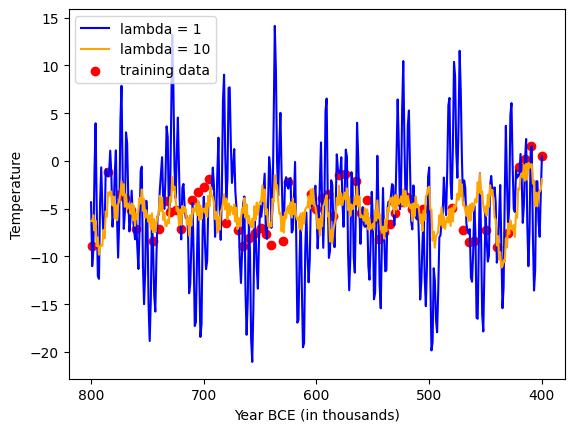
\includegraphics[width=0.75\linewidth]{image.png}
        \end{figure}

        \begin{table}[h]
                \centering
                {\color{blue}
                \begin{tabular}{|c|c|}
                    \hline
                    \textbf{$\lambda$ value} & \textbf{MSE} \\
                    \hline
                    1 & 30.0606 \\
                    10 & 15.6184 \\
                    \hline
                \end{tabular}}
                \label{tab:mse_values}
            \end{table}

        For both $\lambda$ values $1$ and $10$ we see lower mean squared error values of around $30.0606$ and $15.6184$ respectively, compared to the MSE of 58.8855 in basis $(d)$ We can see that the graph in basis $(d)$ is very spiky with lots of variance, and the graphs from LASSO seem to be less so, especially as $\lambda$ increases for $\lambda=10$.
        
	\end{enumerate}
\end{solution}


%%%%%%%%%%%%%%%%%%%%%%%%%%%%%%%%%%%%%%%%%%%%%
% Name and Calibration
%%%%%%%%%%%%%%%%%%%%%%%%%%%%%%%%%%%%%%%%%%%%%
\newpage
\subsection*{Name: Charles Zhou}

\subsection*{Collaborators and Resources}
Whom did you work with, and did you use any resources beyond cs181-textbook and your notes?

I used the Matrix Cookbook and Math for ML book to reference for math such as MVN Guassian and other vector calculus properties.


\end{document}
